\begin{figure}[!b]
\centering
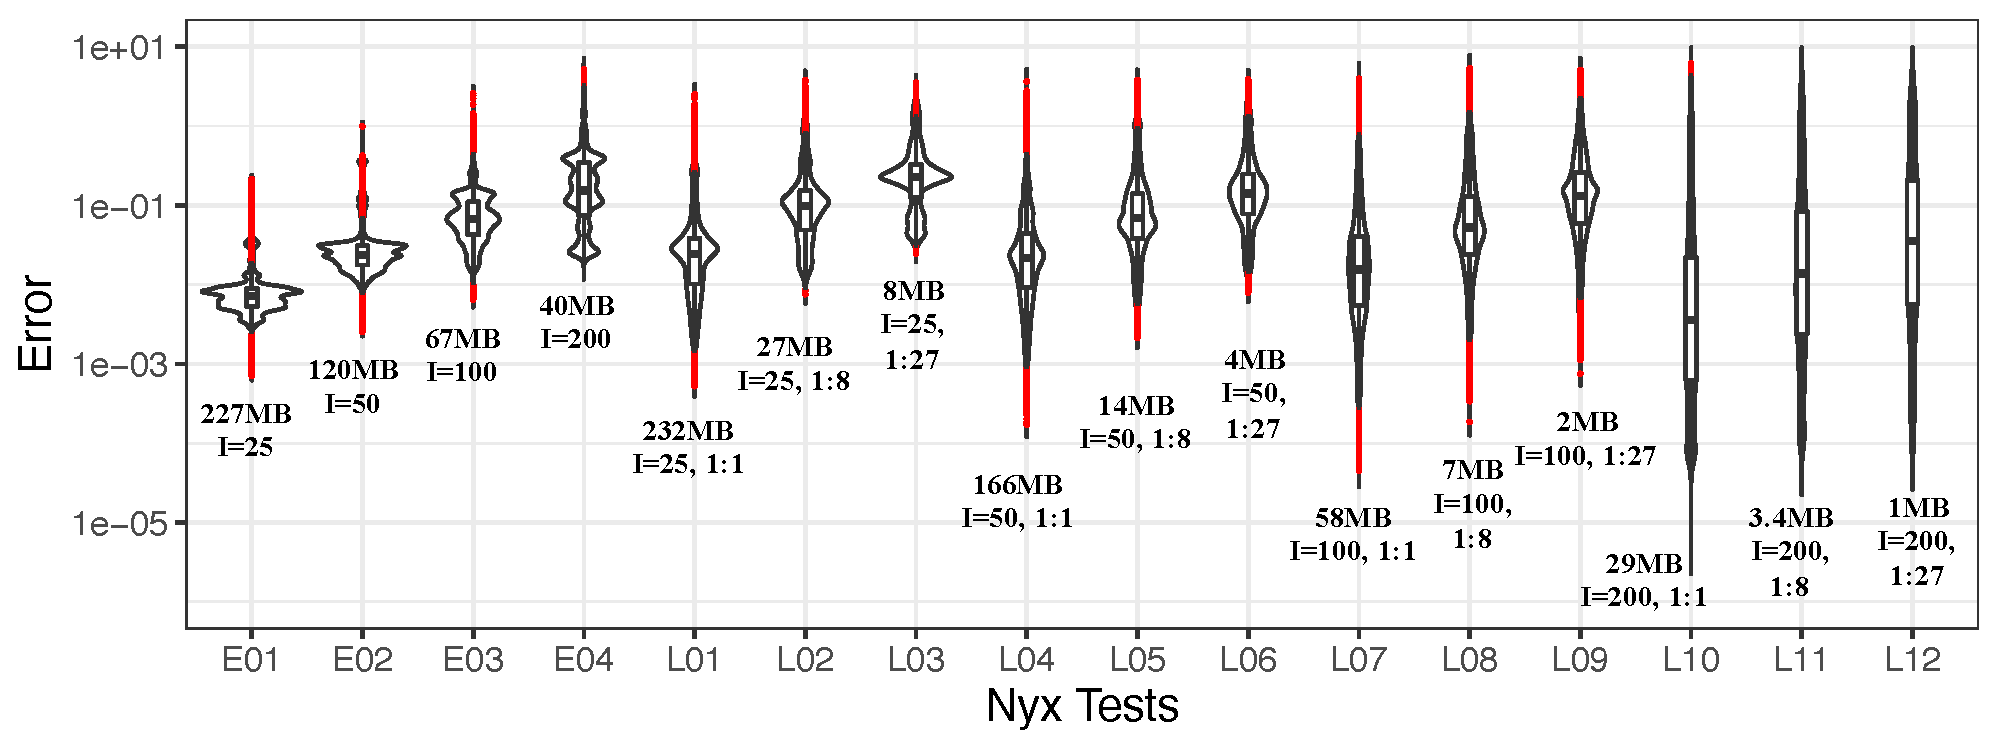
\includegraphics[width=\linewidth]{Images/nyx_violinplot.pdf}
\vspace{-5mm}
\caption{Efficacy results for the Nyx experiments. Each violin plot shows the distribution of the particle reconstruction error for a specific configuration and the horizontal blue dashed line in the chart represents an error equivalent to a single grid cell side. The error axis uses a logarithmic scale. While Eulerian configurations contain greater uncertainty as the value of storage interval \textbf{I} increases, the Lagrangian representations offer the opportunity for improvements in accuracy. Additionally, we find high reconstruction accuracy relies on a high spatial sampling resolution as well.}
\label{fig:nyx_violinplot}
\end{figure}
